% !TEX encoding = UTF-8
% !TEX TS-program = pdflatex
% !TEX root = ../thesis.tex

\chapter{State of the art and technology background}
This chapter presents the pre-concepts needed to comprehend this paper's content fully.
As is understandable from the introduction, they are about Self-Sovereign Identity and 
blockchains. In addition, state of the art will be analyzed to see what has already been
done and what can be improved.
% /*//////////////////////////////////////////////////////////////
%                       TECHNOLOGY CONCEPTS
% //////////////////////////////////////////////////////////////*/
\section{Technology concepts}
This section will explain in detail SSI and blockchain technologies.
\subsection{Self-Sovereign Identity concepts}
Here can be read a brief reprise of what has already been saying about Self-Sovereign 
Identity and a description of its main primitives: VCs, VPs, and DIDs.
\subsubsection{Self-Sovereign Identity}
Self-Sovereign Identity is an approach to digital identity that gives individuals 
control over their data. SSI addresses the difficulty of establishing trust in 
interaction and allows people to interact in the digital world with the same freedom 
and ability to trust as they have in the offline world.
\vspace*{0.3cm}\\
To be trusted, a party in an interaction will present credentials to other parties, 
and those parties can verify that the credentials come from an \textbf{issuer} they trust.
This way, the \textbf{verifier}'s trust in the issuer is transferred to the credential 
\textbf{holder} (or \textbf{prover}). This basic structure of SSI with three participants 
is sometimes called the "triangle of trust.", simply because you need an element of trust
among these entities for them to work together.
\vspace*{0.3cm}\\
While this does not mean that there is a legal partnership or understanding between the 
entities involved, it does mean that each of the entities is willing to examine the 
credibility of the other, and this implicit trust is what constitutes this term.
\begin{center}
    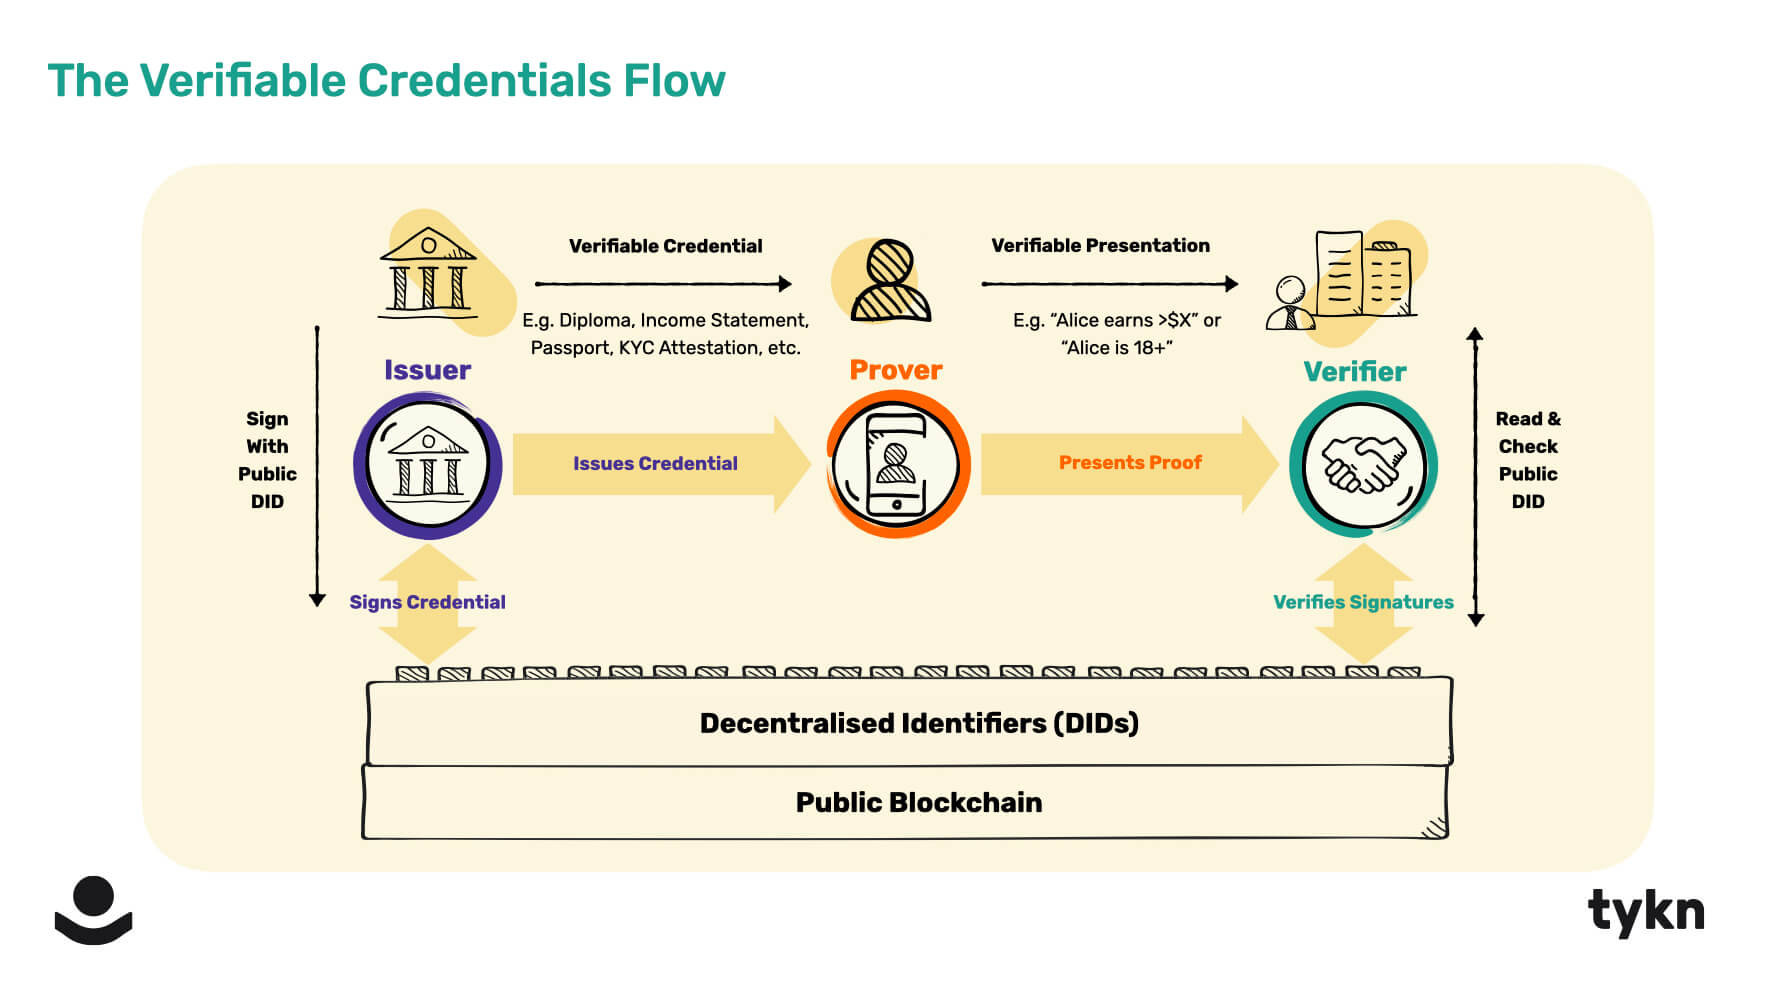
\includegraphics[scale=0.2]{chapter2/triangleTrust2.jpeg}
    \captionof{figure}{The triangle of trust: Prover, Issuer, and Verifier (by Tykn)}
\end{center}
\subsubsection{Verifiable Credential (VC)}
A verifiable credential can represent all of the same information that a physical 
credential represents. The addition of technologies, such as digital signatures, 
makes verifiable credentials more tamper-evident and more trustworthy than their 
physical counterparts.\\
\begin{center}
    \vspace*{-0.5cm}
    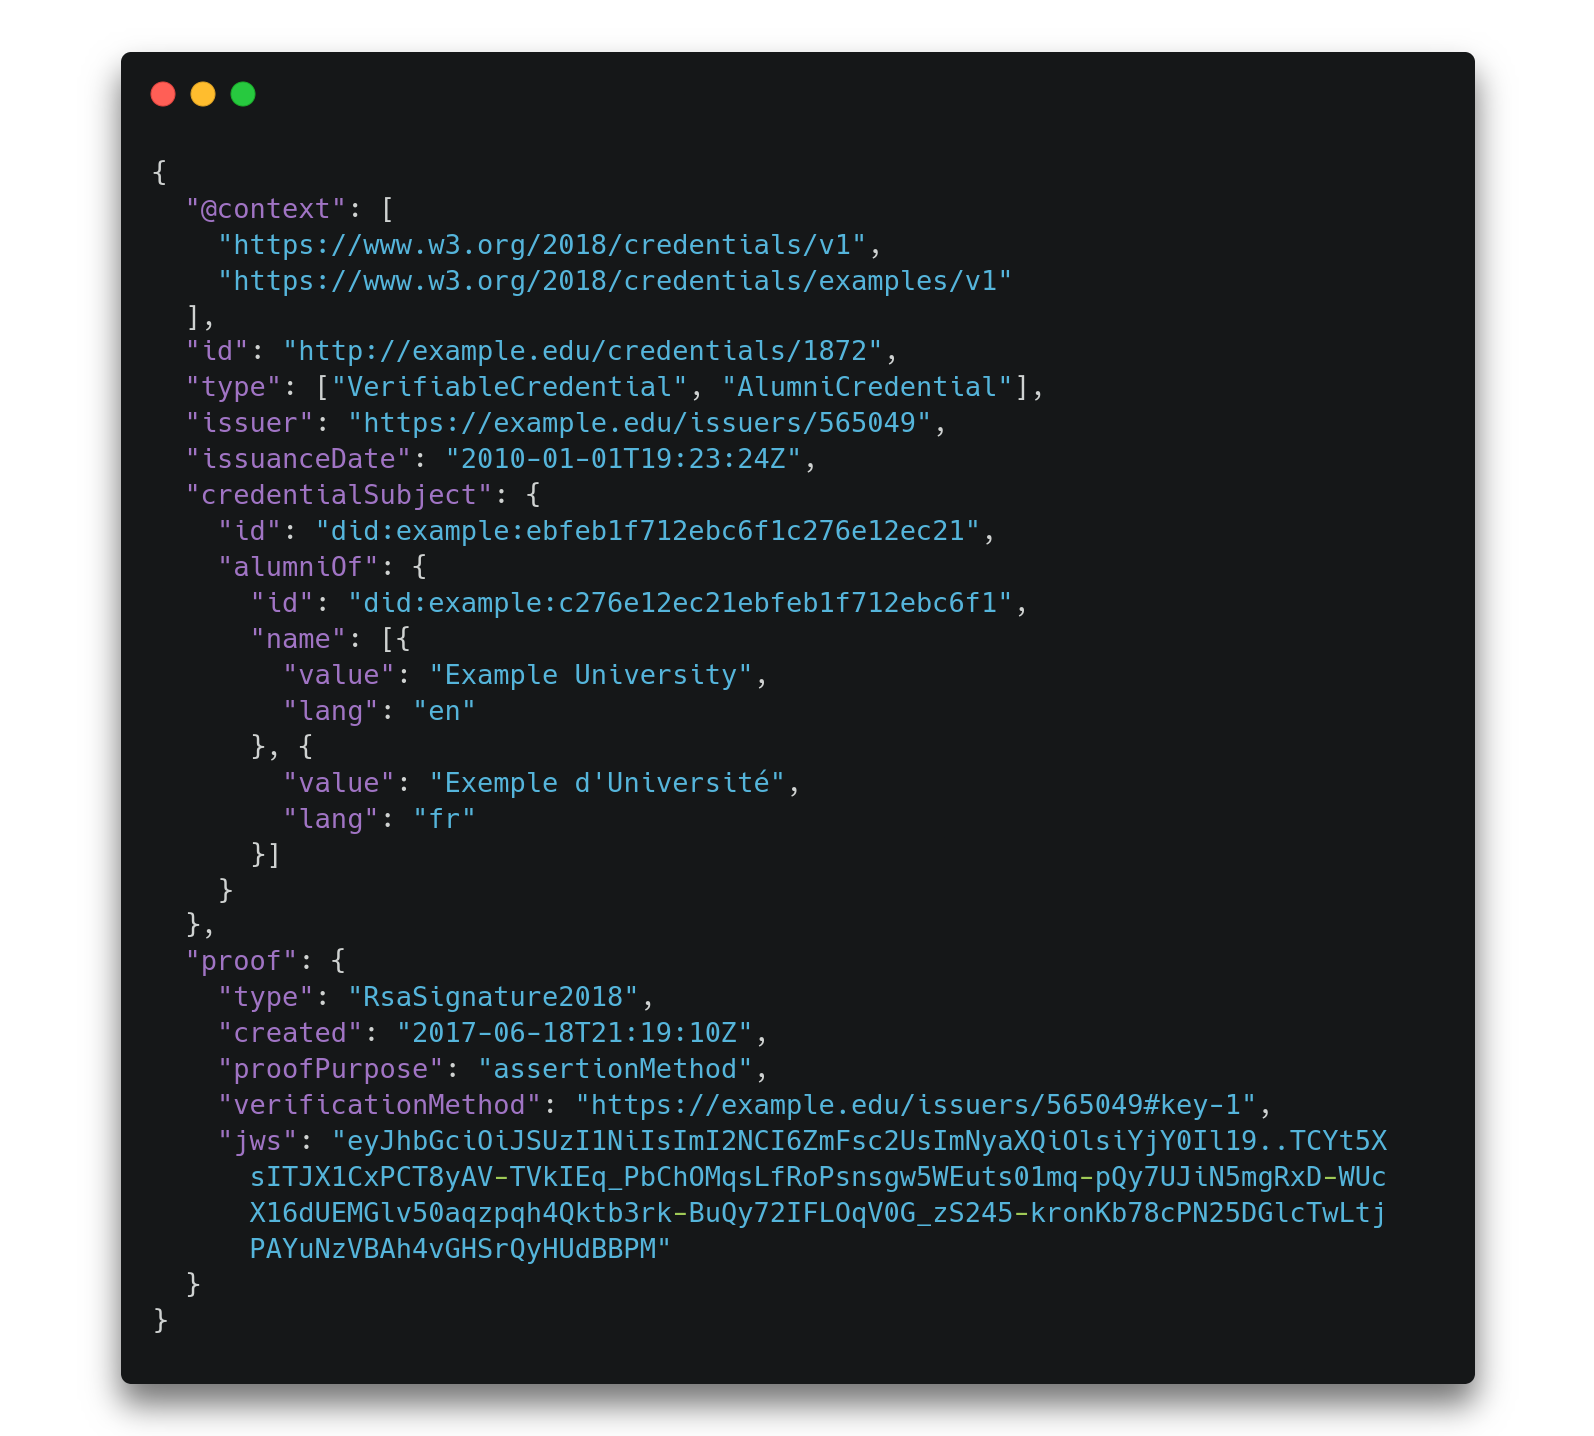
\includegraphics[scale=0.2]{chapter2/exampleVc.png}
    \captionof{figure}{Example of verifiable credential (VC)}
\end{center}
Holders of verifiable credentials can generate verifiable presentations and then share 
these verifiable presentations with verifiers to prove they possess verifiable 
credentials with certain characteristics.\\
Both verifiable credentials and verifiable presentations can be transmitted rapidly, 
making them more convenient than their physical counterparts when trying to establish 
trust at a distance.
The three main components of a VC are:
\begin{enumerate}
    \item \textbf{Metadata}: cryptographically signed by the issuer. It describes the credential
    properties, such as the issuer, the expiry date and time, a public key to use 
    for verification purposes, the revocation mechanism, and other information;
    \item \textbf{Claims}: a statement made about a subject. Example: “Janice’s date of 
    birth is 01/01/1990.”
    \item \textbf{Proofs}: a proof is data about the identity holder that allows others 
    to verify the source of the data (i.e., the issuer), check that the data belongs to 
    (only) the holder, that the data has not been tampered with, and finally, that the 
    issuer has not revoked the data.
\end{enumerate}

\subsubsection{Verifiable Presentation (VP)}
A verifiable presentation expresses data from one or more verifiable credentials and is 
packaged in such a way that the authorship of the data is verifiable. If verifiable 
credentials are presented directly, they become verifiable presentations. Data formats 
derived from verifiable credentials that are cryptographically verifiable but do not 
themselves contain verifiable credentials might also be verifiable presentations.
\begin{center}
    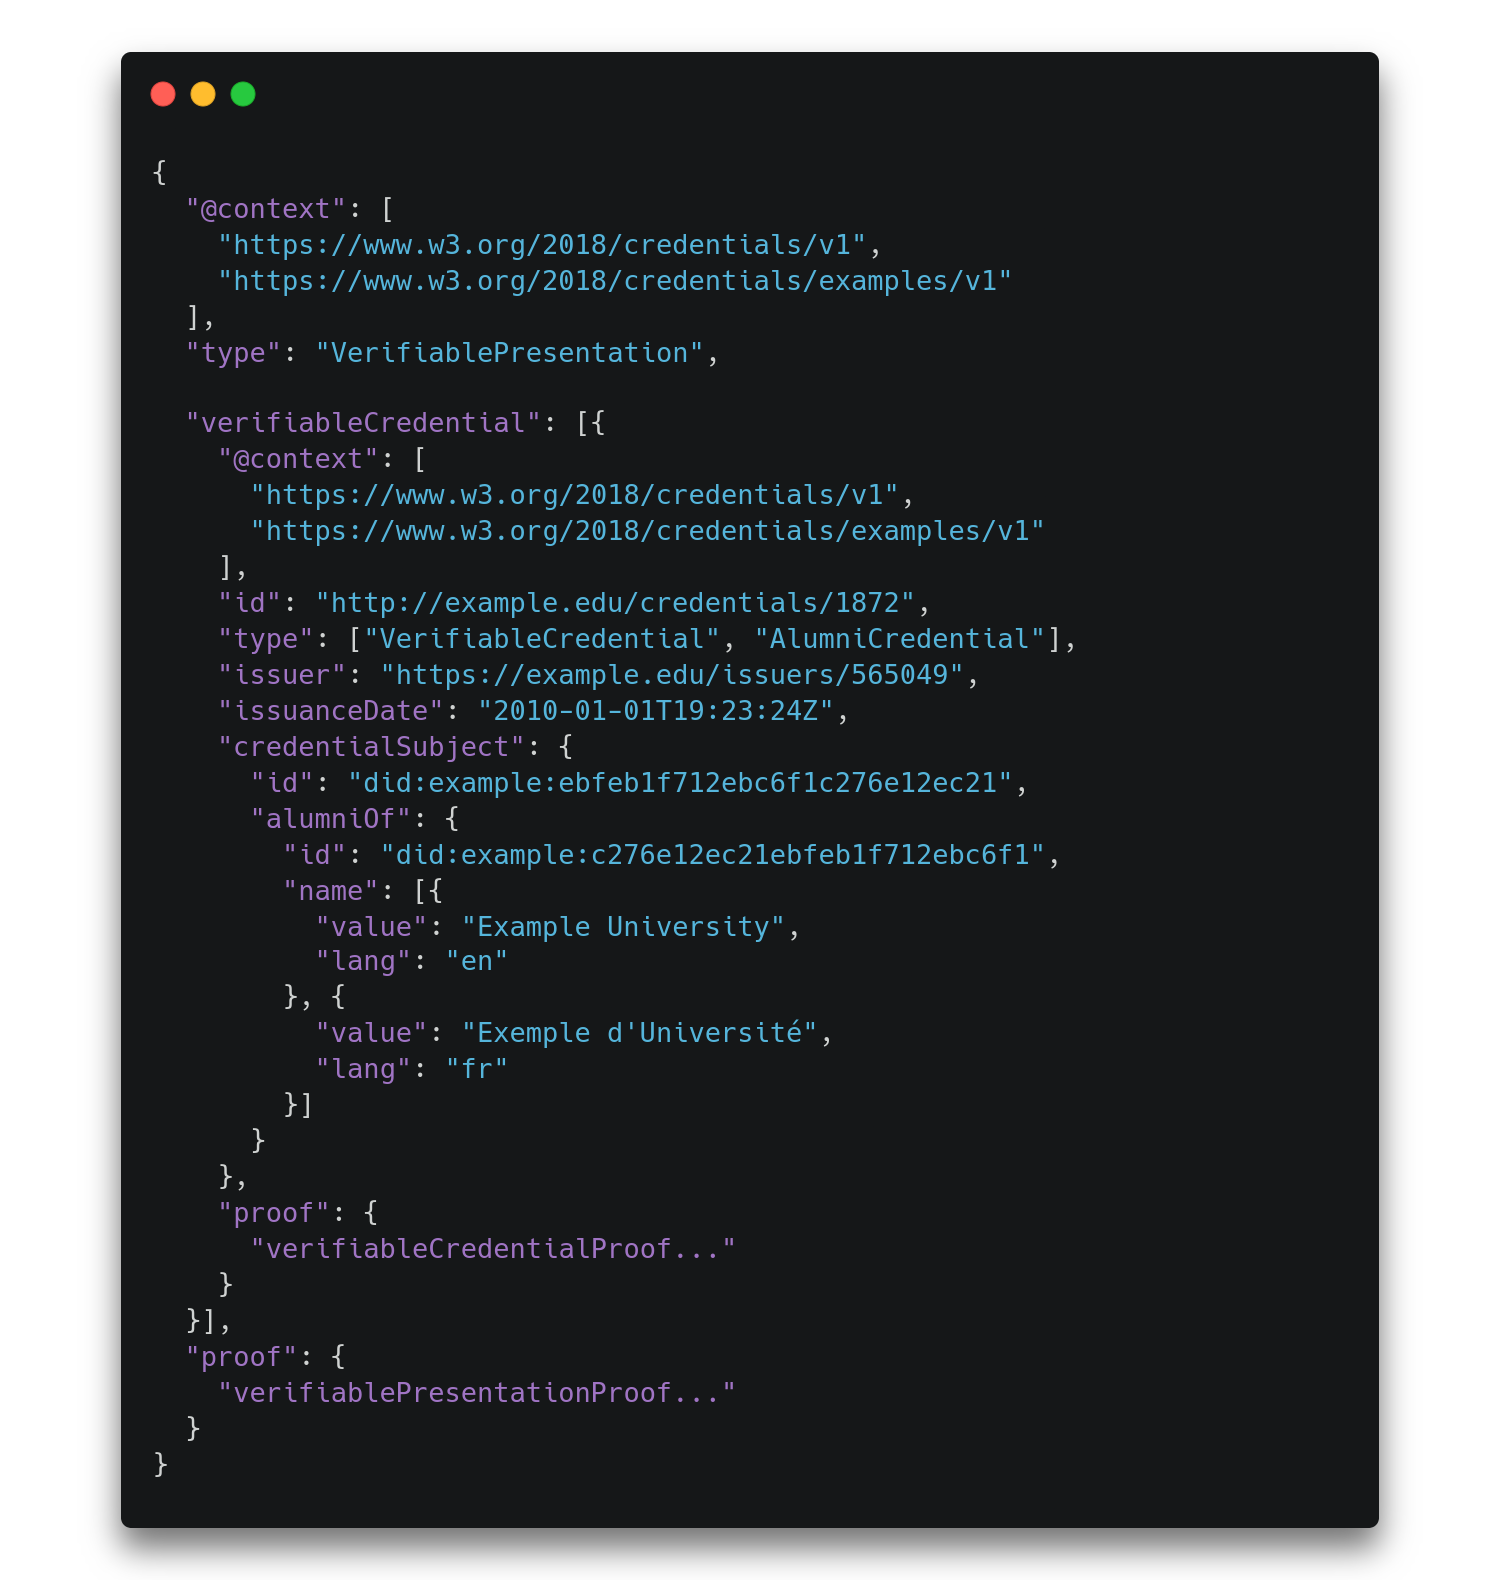
\includegraphics[scale=0.18]{chapter2/exampleVp.png}
    \captionof{figure}{Example of verifiable presentation (VP)}
\end{center}
The data in a presentation is often about the same subject but might have been issued by 
multiple issuers. The aggregation of this information typically expresses an aspect of 
a person, organization, or entity.
\subsubsection{Decentralized Identifier (DID)}
\subsubsection{JSON, JWS and JWT}

\subsection{Blockchain concepts}
\subsubsection{Blockchain}
\subsubsection{Permissionless and permissioned blockchains}
\subsubsection{Bitcoin}
\subsubsection{Ethereum}
\subsubsection{Hyperledger}
\subsubsection{Hyperledger Besu}
\subsubsection{Hyperledger Fabric}

\subsection{Libraries and Stack involved}
\subsubsection{EBSI}
\subsubsection{walt.id SSI Kit}

% /*//////////////////////////////////////////////////////////////
%                        STATE OF THE ART
% //////////////////////////////////////////////////////////////*/
\section{State of the art}
